\chapter{User Documentation}
\label{ch:user}

To ensure optimal performance consistent with testing, the recommended hardware includes an Nvidia GeForce 3050 Ti (with a minimum of 4GB VRAM) and at least 8GB of system RAM. The game is distributed as a ZIP archive specifically for Windows; all necessary files are included, and the game can be launched directly by running the executable. For other operating systems, the game must be built from the provided source files.

Windows does not automatically use the Nvidia graphics card when you run an OpenGL application. You need to manually configure this by navigating to System > Display > Graphics then browse for the game and choose high performance in graphics preference.

\section{The goal of the game}

This project serves mainly as a demonstration of the implementation so no complicated features are implemented. However, to make the game playable the user is assigned with a single task. The goal of the game is drop packages at some predefined coordinates which are randomly selected as soon as the package is dropped. The package can be dropped in some predefined circle of radius around the target coordinates. So the steps can be summarized as: 

\begin{itemize}
	\item Fly around and explore the world.
	\item Fly to the target coordinates.
	\item When you see a sign on the screen, drop the package. And go to the next coordinates.
	\item Settings can be manually configured as desired, which change the shape and scale of the clouds.
	\item The airplane's properties can also be configured using the menu.
\end{itemize}

A navigation bar is also added at the bottom of the screen which is just a projection of the players coordinates on the $x$-$z$ plane, this bar can be used for reaching the target coordinates as will be momentarily described.

\section{Playing the game}

\begin{figure}[H]
    \centering
    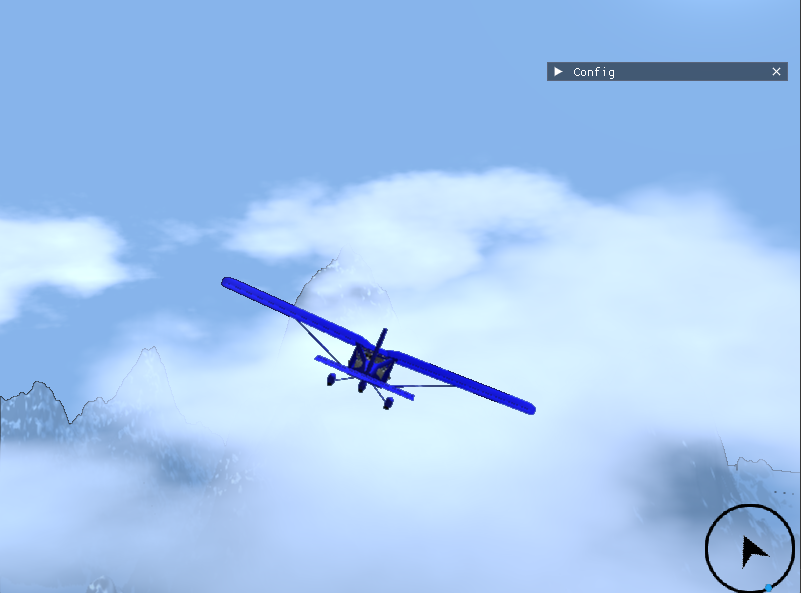
\includegraphics[width=0.75\textwidth]{images/game1.png}
    \caption{First look}
    \label{fig:first-look}
\end{figure}


The image above provides a first look at the game, the config menu can be hidden using either the cross button or by pressing the key \textbf{F1}. Currently there is no way to change the airplane model from inside the game, the only way to do that is to change the source files.

\bigskip

\subsection{The controls}

Following keys can be used to control the aircraft:
\begin{compactdesc}
  \item[\textbf{W}:] Go forward (apply thrust)
  \item[\textbf{D} or $\rightarrow$:] Tilt the plane towards right.
  \item[\textbf{A} or $\leftarrow$:] Tilt the plane towards left.
  \item[$\uparrow$:] Tilt the plane downwards.
  \item[$\downarrow$:] Tilt the plane upwards.
  \item[\textbf{space-bar}:] Drop the package
  \item[\textbf{Q}:] Rotate the aircraft around the UP axis to the left.
  \item[\textbf{E}:] Rotate the aircraft around the UP axis to the right.
\end{compactdesc}


\subsection{Understanding the navigation bar}
The navigation bar can be understood by looking at the picture below
\begin{figure}[H]
    \centering
    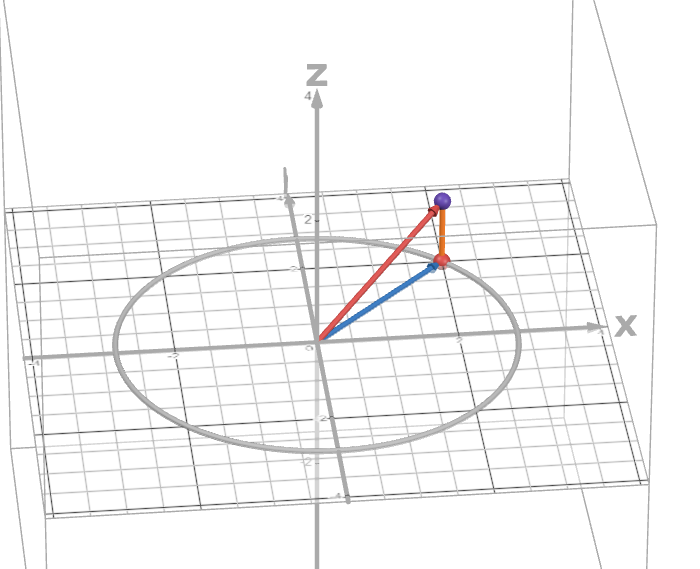
\includegraphics[width=0.75\textwidth]{images/figure1.png}
    \caption{Projection of a point in 3d onto the plane}
    \label{fig:projection}
\end{figure}


If the vector in red is current velocity vector of the airplane and the blue vector is its projection onto the horizontal plane then this vector is exactly where the black arrow points in the navigation bar.

The blue blinking dot is where the current target position is, it is relative meaning that the distance is scaled and capped so it remains within the navigation bar but if you're closer to the target then the blue point moves inside the circle indicating that you're near the target.

\subsection{Dropping the package}

When you are within the pre-specified acceptable radius of the target a text as show in Figure~\ref{fig:drop_text} appears on the screen.

At which point you can press \textbf{space-bar} to drop the package and move to the next assigned point in the navigation bar.


\begin{figure}[H]
    \centering
    
\includegraphics[width=0.5\textwidth]{images/figure2.png}
    \caption{Text indicating the drop point}
    \label{fig:drop_text}
\end{figure}



\section{Understanding the config menu}

\begin{figure}[H]
	\centering
	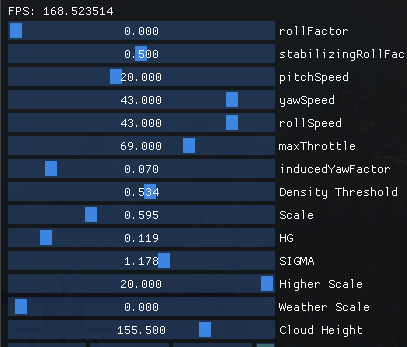
\includegraphics[width=1.0\textwidth,height=0.5\textheight,frame]{images/figure3.png}
	\caption{The configuration menu}
	\label{fig:config_menu}
\end{figure}

The first 7 configuration parameters (until \textbf{inducedYawFactor}) are for the aircraft. And they control/define the following things:


\begin{center}
	\begin{longtable}{ | p{0.3\textwidth} | p{0.7\textwidth} | }
		
		\hline
		\multicolumn{2}{|c|}{\textbf{Aircraft parameters}}
		\\ \hline
		
		\emph{Parameter} & \emph{Description}
		\\ \hline \hline
		\endfirsthead % table header on first page
		
		\hline
		\emph{Parameter} & \emph{Description}
		\\ \hline \hline
		\endhead % table header on further pages
	
		\hline
		\endfoot % table footer on previous pages
		
		\endlastfoot % table footer on last page
		
		\emph{\textbf{rollFactor}}
		& How much emphasis should be put on the roll control given by the user, the total roll torque is a weighted sum of user's roll and the stabilizing roll.
		\\ \hline
		
		\emph{\textbf{stabilizingRoll}}
		& How much emphasis should be put on the stabilizing the aircraft, for example, if the aircraft is traveling fast it has a tendency to align itself towards the center, this parameter controls how strongly that should happen.
		\\ \hline
		
		\emph{\textbf{pitchSpeed}}
		& Factor by which changes to the current pitch should be applied. 
		\\ \hline
		
		\emph{\textbf{yawSpeed}}
		& Factor by which changes to the current yaw should be applied. 
		\\ \hline
		
		\emph{\textbf{rollSpeed}}
		& Factor by which changes to the current roll should be applied. 
		\\ \hline
		
		\emph{\textbf{maxThrottle}}
		& Factor by which the force in the forward direction should be applied when the user presses \textbf{W}
		\\ \hline
		
		\emph{\textbf{inducedYawFactor}}
		& When the airplane tilts around the $z$ axis, i.e it rolls there is also an induced yaw on it, this parameter determines how strong that induced yaw should be. 
		\\ \hline
		
		\caption{Aircraft parameters}
		\label{tab:aircraft_params}		
	\end{longtable}
\end{center}



\begin{center}
	\begin{longtable}{ | p{0.3\textwidth} | p{0.7\textwidth} | }
		
		\hline
		\multicolumn{2}{|c|}{\textbf{Weather parameters}}
		\\ \hline
		
		\emph{Parameter} & \emph{Description}
		\\ \hline \hline
		\endfirsthead % table header on first page
		
		\hline
		\emph{Parameter} & \emph{Description}
		\\ \hline \hline
		\endhead % table header on further pages
	
		\hline
		\endfoot % table footer on previous pages
		
		\endlastfoot % table footer on last page
		
		\emph{\textbf{Density Threshold}}
		& The clouds have density between 0 and 1 at points in space, this determines the minimum density the point must to have to be rendered.
		\\ \hline
		
		\emph{\textbf{Scale}}
		& The scale at which the clouds should we sampled from the noise textures, lower values result in bigger fluffier clouds, higher values make them smaller and closer.
		\\ \hline
		
		\emph{\textbf{HG}}
		& The Henyey-Greenstein constant (further described in developer documentation).
		\\ \hline
		
		\emph{\textbf{SIGMA}}
		& The transmittance factor of the clouds.
		\\ \hline
		
		\emph{\textbf{Higher Scale}}
		& The scale at which noise from high frequency noise textures should be sampled from. Empirically, this was found to give good results between 15 and 20.
		\\ \hline
		
		\emph{\textbf{Weather Scale}}
		& The scale at which the parameters for the weather (i.e where clouds can be) should be sampled from the weather texture (due to the noise textures I have, this value should be extremely small).
		\\ \hline
		
		\emph{\textbf{Cloud Height}}
		& Height at which the clouds should be.
		\\ \hline
		
		\caption{Weather parameters}
		\label{tab:weather_params}		
	\end{longtable}
\end{center}



\begin{center}
	\begin{longtable}{ | p{0.3\textwidth} | p{0.7\textwidth} | }
		
		\hline
		\multicolumn{2}{|c|}{\textbf{Terrain Parameters}}
		\\ \hline
		
		\emph{Parameter} & \emph{Description}
		\\ \hline \hline
		\endfirsthead % table header on first page
		
		\hline
		\emph{Parameter} & \emph{Description}
		\\ \hline \hline
		\endhead % table header on further pages
	
		\hline
		\endfoot % table footer on previous pages
		
		\endlastfoot % table footer on last page
		
		\emph{\textbf{Draw Water}}
		& Draw water over the terrain, the default height is 5.0 (not alterable).
		\\ \hline
		
		\emph{\textbf{Draw Normals}}
		& Draw normals for the terrain, the default color is white (not alterable).
		\\ \hline
		
		\emph{\textbf{Line Mode}}
		& Draw the terrain in line mode (just the edges of the triangles), to see the effects of LOD.
		\\ \hline
				
		\caption{Terrain Parameters}
		\label{tab:terrain_params}		
	\end{longtable}
\end{center}